\section{Mechanisms} \label{section:mechanisms}
\subsection{Recovery System}  % TODO: requirement links

As discussed earlier in this report, we are currently unsure whether the first stage of the space\-shot vehicle will be expended. For this reason, we are designing systems to safely recover both stages (MEC.2), with the understanding that the first stage recovery system may be removed in the future.

For the second stage of the rocket, descent speeds are not to exceed 50 feet per second above 1000 feet in altitude, and must not exceed 20 feet per second below 1000 feet to keep the more sensitive structures of the vehicle intact (MEC.2.2). Under the assumption that the booster stage also needs to be recovered, it has a similar set of requirements, though the allowable velocities will be some amount higher since it is expected that the first stage will be more durable and more able to withstand a hard landing (MEC.2.1). Depending on the booster recovery design selected, this velocity will likely range between 20 and 40 feet per second.

The recovery systems for each stage will deploy from a single airframe separation in each of their respective airframes (MEC.2.1.2 and MEC.2.2.2). Prior to separation, each of the airframe sections will be held together through the use of nylon shear pins. The booster recovery system will deploy from a break in the airframe between the motor and the staging interface. The sustainer recovery system will deploy from a break above avionics and below the nosecone. Due to the high altitude of both recovery deployments, a simple separation mechanism will be used to break apart the airframe (MEC.2.1.2.1 and MEC.2.2.2.1). The specifics for this device are found later in \Cref{section:sep-mech}.

\subsubsection{First Stage Recovery} %TODO: fix overfull hbox
Two minimal recovery designs for the first stage are being considered, in case it is determined that the first stage must not be expended. Line diagrams for all the recovery schemes discussed in this report are provided in \Cref{section:line-dia-appendix}, for further reference. The first design consists exclusively of a separation mechanism, one line of shock cord approximately twice the length of the booster, and a mid-sized parachute. This option is intended to be extremely compact and lightweight to allow for minimal design work by the structures and avionics teams. As only a single chute is used for this design, descent speeds will be much higher than the ideal 15 to 20 feet per second below 1000 feet. Descent speeds will likely range between 30 and 40 feet per second for the entirety of the descent to prevent excessive drift from the stage’s apogee. The landing impact for the booster will be more forceful than what a typical recovery system would result in, but we currently expect the booster to be tough enough to withstand the conditions without severe damage. Since no valuable payload is onboard, this rough landing is deemed acceptable.

The second parachute option we are considering is a ``Sombrero''. This device is a mini\-/parachute attached to the canopy cords, which is able to freely slide up and down, allowing the main chute to unfurl roughly depending on its position. Early estimates indicate this system could use only five times the rocket length in shock cord compared to the nine times used by a conventional drogue-main setup. Acquiring one may be difficult, as the ``Sombrero'' is a patented device created by Butler Parachutes. They do offer custom orders for parachute systems, but pricing is unknown and requires further inquiry. Another option would be to manufacture a similar system in-house, but that leads to risk of the device being of poor quality and failing during use. This parachute system offers a great way to reduce mass and volume, but it is difficult to source or manufacture.

While the two recovery systems are similar, they each pose their own advantages and disadvantages. The single chute alone is by far the simplest, most reliable, lightest, and cheapest method, but it has the booster landing at a high velocity of 30 to 40 feet per second. This will undoubtedly damage the booster to some extent, but it is likely to remain in one piece. Also, it is not likely to bury itself in the launch range, allowing for it to be easily located and retrieved. The sombrero avoids a hard impact, but it is significantly more difficult to manufacture, is far more expensive, and adds more mass to the rocket. Further research will be conducted into both systems to choose an ideal option.


\subsubsection{Second Stage Recovery}
There are also two options for second stage recovery systems. Line diagrams for these options are provided in \Cref{section:line-dia-appendix}. The first option is the most massive as it requires 8-9 times the length of the sustainer in shock cord. However, currently it is deemed the most reliable method, and the team has the most experience with this system as similar recovery designs have been used for two of our previous flights. This method uses a traditional drogue-to-main parachute scheme. At apogee, the separation mechanism separates the single sustainer airframe break and deploys the drogue parachute, also releasing the main parachute bundled in a parachute bag. A single line of shock cord will run from the drogue parachute to the rocket body where it is attached by use of a tender descender. A tender descender is a simple device that holds two quick links together until a black powder charge that was previously contained within the device detonates in response to a signal from the avionics computers. This line connecting the drogue to the tender descender will carry all of the chute tension above 1000 feet in altitude. During descent, the drogue will slow the rocket down to acceptable speeds around 50 feet per second before the system reaches 1000 feet in altitude. Shock packs, various devices that reduce the high forces of parachute deployment or snatch force, will be implemented throughout the system to limit stress on mechanical mounting structures during descent. 

Running parallel to the tender descender to drogue shock cord during the entirety of the descent above 1000 feet will be a secondary set of shock cords which connect the main chute to both the drogue chute and the rocket body. This shock cord will use a different mounting location than the tender descender. Above 1000 feet, this system will be in slack, and the main parachute will be contained within its bag. At 1000 feet, the tender descender holding the force of the drogue chute will separate, transferring the path of tension through the shock cord connected to the main chute. This tension will rapidly remove the main chute from its bag as the rocket body falls away from the drogue parachute. As the path of tension will transfer from the rocket, to the main, and then to the drogue, the upward force of the drogue will help to quickly inflate the main parachute. The deployed main parachute will then bring the rocket descent speed down to a gentle 15 to 20 feet per second. 

For the sustainer stage recovery, the second recovery option that is being researched is reefing parachutes. This system consists of a main chute that can be variably deployed by temporarily fixing the shroud line length via a reefing ring. Essentially, this system allows the single parachute to act both as the drogue and the main chute. This system would greatly decrease the amount of shock cord required to roughly four times the length of the rocket and entirely eliminate the need for a drogue chute, saving valuable mass and volume. Also, if only one chute is used, it would reduce the snatch force the rocket would experience, compared to deploying a chute in the standard fashion.  However, as a team, we lack experience using this system and creating or sourcing a reefed chute has an unknown price tag or level of reliability.

After researching several reefing options, the following are being considered:

\raggedright\begin{enumerate} % TODO: fix overfull hbox
    \item Single reefing ring: simplest option, but not too predictable especially at high altitudes.
    \item Double reefing ring configuration: Using friction, we can delay the opening process of the parachute. We still need to further study this option.
    \item Active reefing process: Using a triggered event from avionics to loosen or drop the reefing ring, allowing the chute to expand from a drogue to a main at a specified altitude. This option requires significantly more research.
\end{enumerate}

As it contains 8 to 9 times the length of the rocket in shock cord, two chutes and a tender descender, the first recovery method mentioned, is by far the heaviest and least space-efficient option. However, this is the option the team has the most experience with, is more reliable, and is easier to manufacture and assemble. The reefing method will take up approximately half of the volume of the first option, immediately making it a strong contender. Various methods of reefing will continue to be explored and tested, but at this time the reliability and feasibility of this much more compact method is still in question.


\subsection{Separation Mechanism} \label{section:sep-mech}
Due to the high altitude required of the recovery deployments for both stages of this vehicle, traditional black powder airframe separations are not viable. These simple systems require atmospheric pressure to both fill the airframe with compressed gas and provide a medium for heat transfer to ignite nearly all of the black powder used in the initial charge. In the low pressure environments in which this rocket will require an airframe separation, another solution is needed (MEC.2.1.2.1 and MEC.2.2.2.1). As recovery systems using tender descenders will not require their use above 1000 feet in altitude, the operation of tender descenders will not be impacted by these same concerns. 

Many rockets flying at these high altitudes use a compressed CO\(_2\) separation system for airframe separation. This technique was researched, but CO\(_2\) canisters and the various systems used to release the gas and separate the airframe are rather bulky, heavy, and relatively complicated which could lead to various points of failure. Since two separation systems could be required for the rocket, this method was deemed unsatisfactory. Instead, a simple black powder piston-like device was designed. A preliminary CAD model of this device is shown in \Cref{figure:sep-cad}. This device consists of a mounting plate, a compartment of O-ring sealed atmosphere within a piston like chamber, a pushing plate, and a firebolt.

A firebolt is simply a bolt that has had a hole drilled through it to allow for the passage of e-match electronic ignitors through the bolt. These e-matches are then sealed within the bolt through the use of epoxy and a small sealed container of  about 0.5 grams to 1 gram of black powder is placed around the ignitor tip of the e-matches. The exact amount of black powder will be determined through on the ground testing of the system long before launch. The threads of the bolt can be wrapped with pipe sealant and placed within the device to form a proper seal, leaving the black powder on the inside of the separation mechanism and the e-match leads on the other end. These leads will be connected to the avionics computers which will then be able to ignite the black powder at a specified time or altitude. As the black powder is contained within a small pocket of atmospheric pressure at any altitude, proper ignition is possible and the separation mechanism will separate itself and the airframe of the rocket in the process.

\begin{figure}
    \centering
    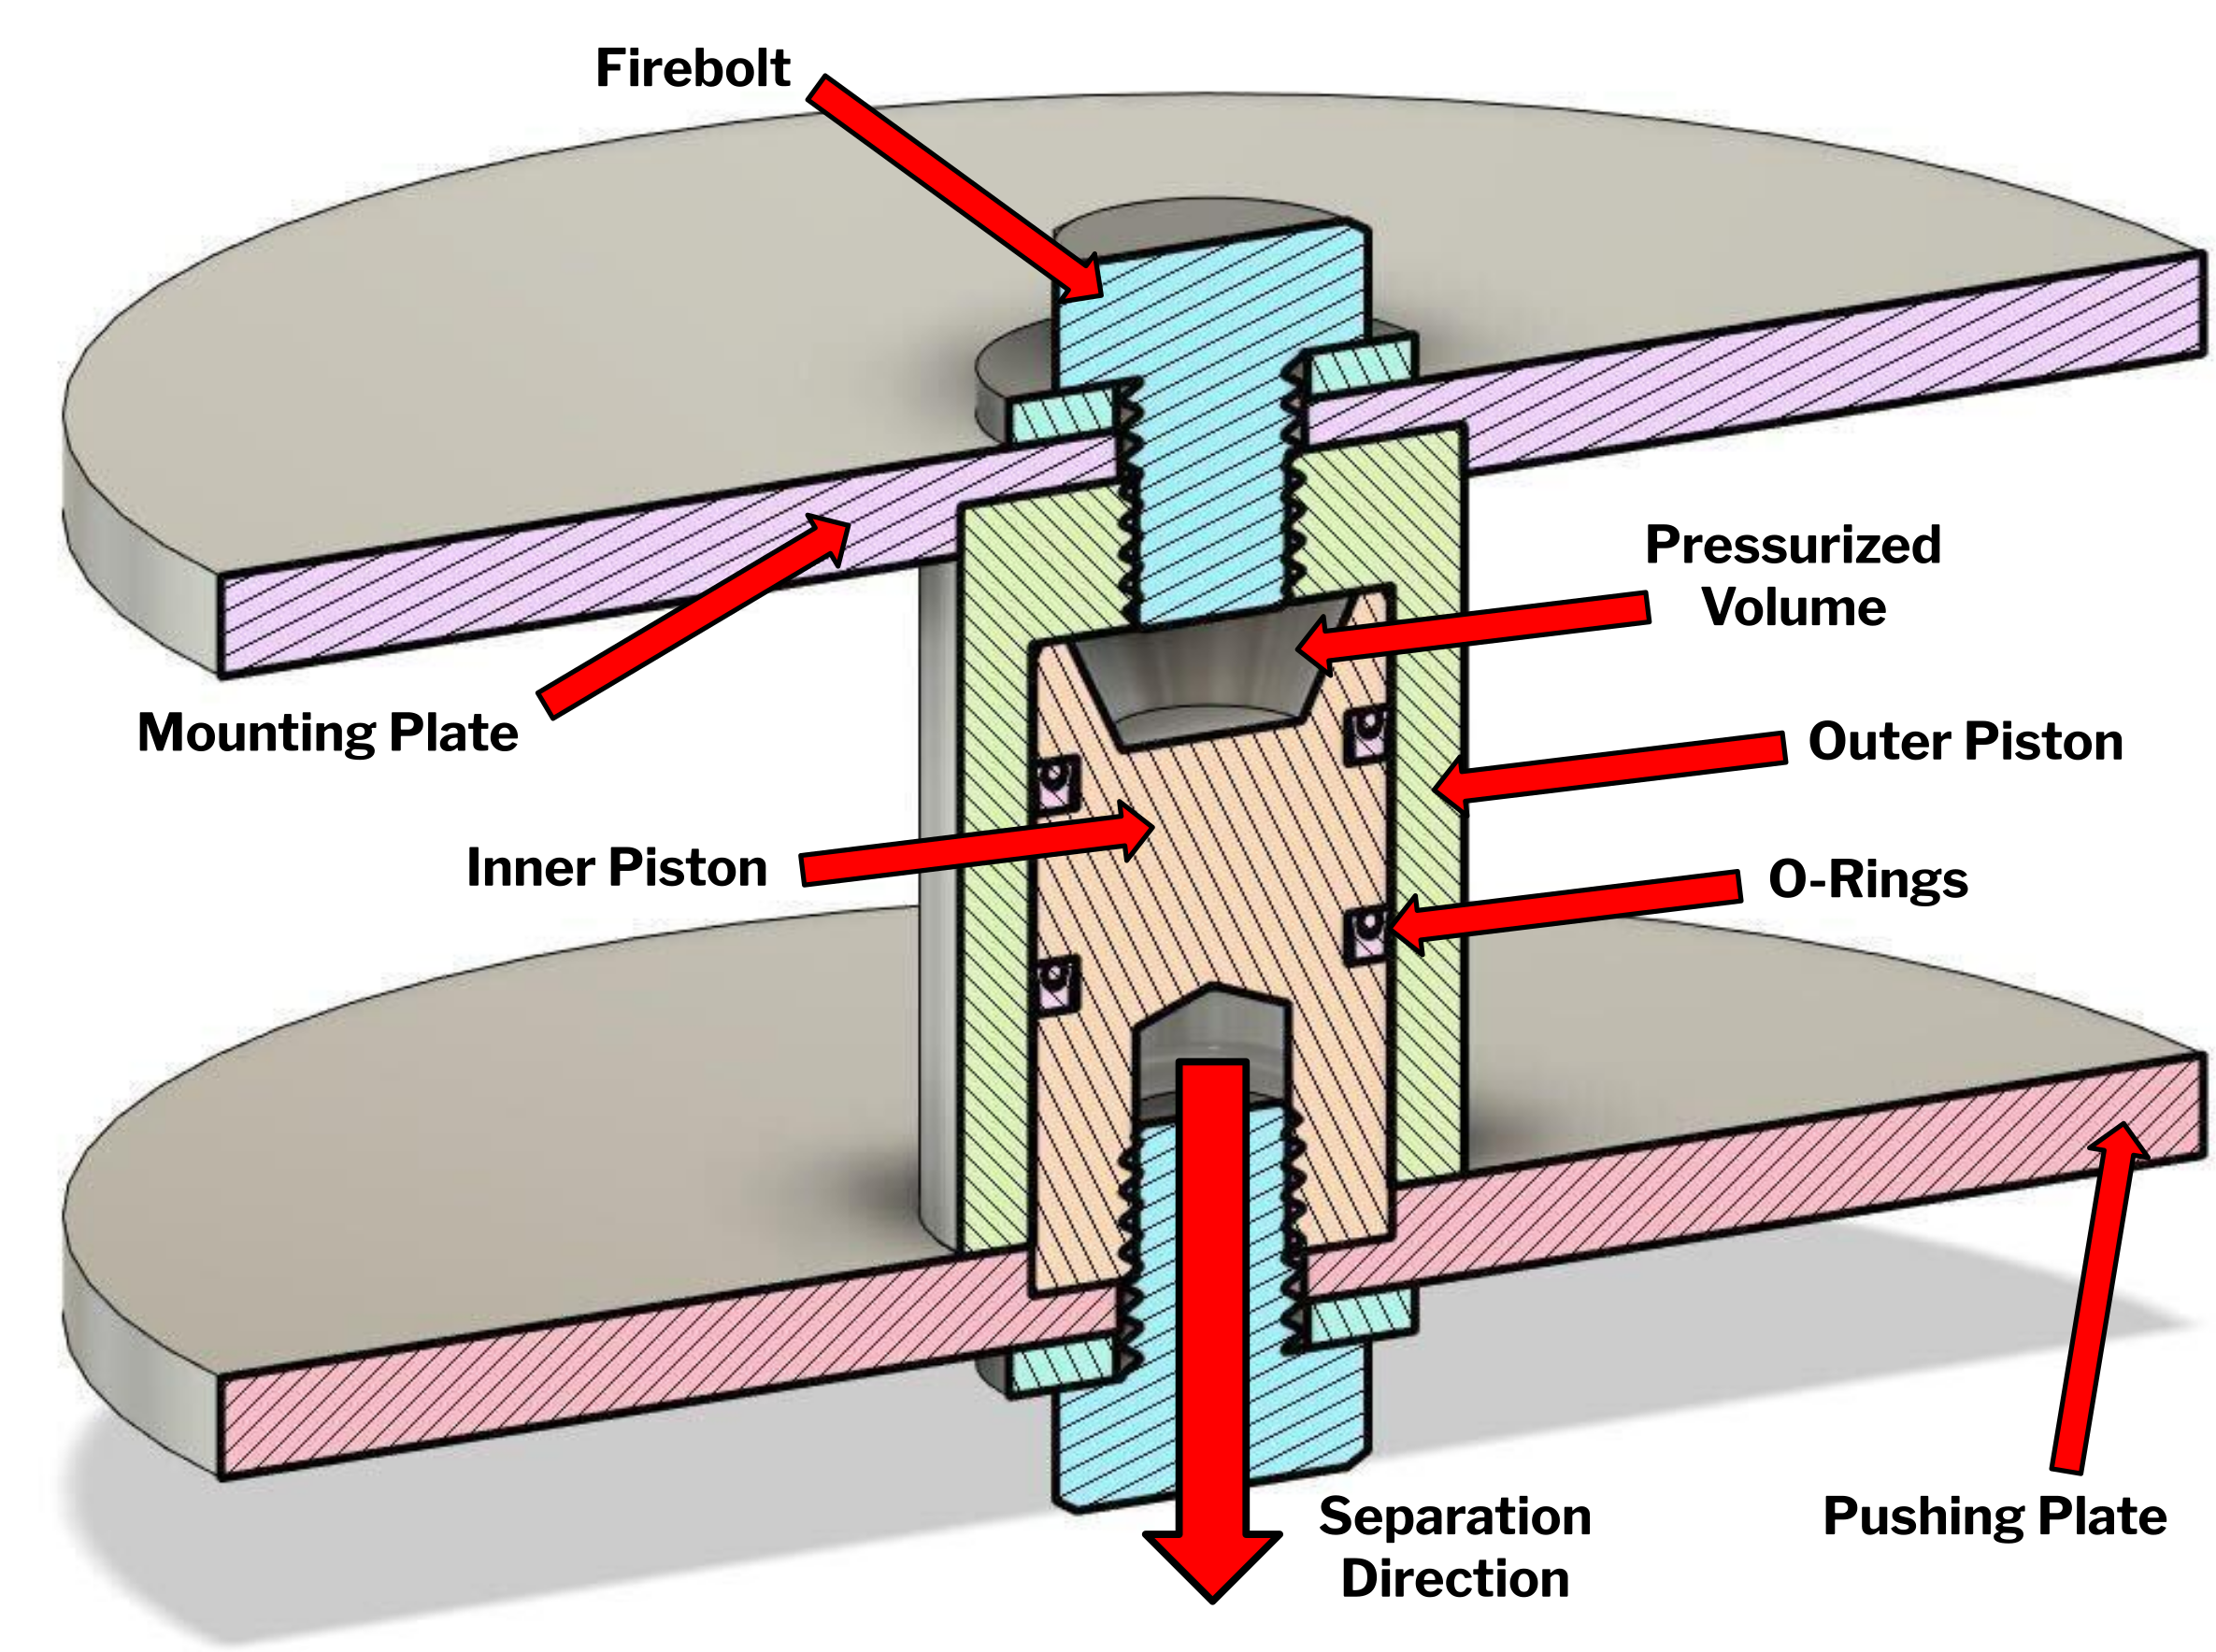
\includegraphics[width=0.8\linewidth]{images/sep-cad}
    \caption{CAD model of the preliminary piston-based separation device}
    \label{figure:sep-cad}
\end{figure}

To actually achieve separation of the airframe, the black powder ignition will force the inner piston upwards relative to the rocket. This movement will be transferred to the airframe coupling through the use of the pushing plate. Since the coupling is attached to the upper half of the airframe and the mounting plate of the separation mechanism is attached to the lower airframe, this force will push the airframe apart.

Two separation mechanisms will be included in the entire rocket if the first stage is required to be recovered: one in the booster stage and one in the sustainer. In both cases, the separation mechanism will be located directly below the parachute bay and above the avionics bay. This allows for easy and safe wiring of the firebolt to the avionics computers. During final rocket assembly, the connection of the two halves of the piston will be the final step, leaving any accidental ignition of the black powder free to expand safely without causing harm to the assembly team or equipment.


\subsection{Inter-Stage Mechanism} \label{section:interstage-mech}

An essential part of the rocket's flight is the clen separation of the two stages between their burns. Since a failure to separate would very likely lead to catastrophic mission failure, it was decided that a stage separation mechanism would need to be developed to satisfy MEC.3.

After preliminary development and research, we concluded that the main separation mechanism should be as simple as possible. The optimal time to separate, based on minimzing the loss of velocity due to drag, is when the two stages would naturally drag-separate, i.e. the drag on the first stage ``pulls'' it off the second stage. However, we are unable to simulate the complex aerodynamics of two free bodies in proximity. Thus, the separation scheme we propose is as follows.

\begin{enumerate}
    \item The first stage burns out
    \item The optimal time of separation occurs. Depending on the aerodynamics of the vehicle, this may occur immediately after first stage burnout. Additionally, the stages may not naturally drag-separate at this point
    \item If the stages do not naturally drag-separate, we will ignite the upper-stage motor, to ``hot-separate'' the stages
    \item Either from the hot separation, or after a short coast after drag-separating, the second stage burn begins
\end{enumerate}

We considered using a mechanism to retain the stages together until the ignition of the upper stage. Shear pins were the leading candidate for this. However, there are potential stability concerns with hot-separating with shear pins. Specifically, if one shear pin breaks even a fraction of a second before the others, a strong moment will be put on the vehicle, disturbing it from its trajectory while the second stage motor is firing. This is unacceptable, so we decided the two stages would simply be nested into each other geometrically, with only a small amount of friction to overcome to stage. Using this separation scheme allows the rocket to be reduced in mass, as no extra mechanism is required in order for the stages to separate. This also saves on cost, as no extra materials are needed. Additionally, it would still keep the second stage stable during separation, allowing the second stage to continue on course as predicted. 

A concern of ours with this scheme is that the uncertainty of the natural drag separation leads to imprecision in our simulation. However, we plan to mitigate this by running simulations where the stages drag-separate immediately after burnout, and simulations where the stages remain together until the second stage ignition.


\subsection{De-Spin Mechanism}
While many rockets with similar missions to ours spin-stabilize, we are not yet able to determine if we will need to. While that uncertainty exists, we have been examining the feasibility of de-spin systems. To satisfy other needs of the mission, namely recovery and payload concerns, the vehicle must be rolling at a rate no higher than 60 revolutions per minute when it reaches apogee (MEC.1). At this point, our analysis has assumed a very large range of possible initial spin rates, between 50 and 1000 revolutions per minute. Of course, as the stability analyses develop, this range will be tightened. After researching the common options for despin, the mechanisms that the team considered were yo-yo despin, cold gas thrusters, hot gas thrusters, and a reaction wheel system.

Yo-yo despin is achieved by wrapping two cables, each attached to a mass, around the rocket. A release mechanism allows the cords to unwind at the desired time, allowing the masses to spread out to the full length of the rope which increases the rocket’s moment of inertia. When the cords are fully extended, they release from the vehicle, carrying a significant amount of angular momentum. Additional optimizations can be done, such as using cables with elasticity, but our preliminary analysis was done with the most basic model. Yo-yo despin is relatively simple, and requires only a small amount of mass and volume.

Cold and hot gas thrusters operate on similar principles. Two small nozzles are aimed tangentially to the airframe, and exhaust gasses are ejected, slowing the rotation of the vehicle. Cold gas thrusters are fuelled by a tank of compressed gas, typically nitrogen or carbon dioxide, while hot gas thrusters use small solid rocket motors to generate the exhaust gas. For both cases, we considered only passive systems with fixed amounts of impulse; a more complex system might, for example, close the valve between the tank and the nozzles when the rotation rate slows sufficiently.

Finally, a reaction wheel would also be capable of reducing the spin of the vehicle by using a motor to spin a flywheel inside the stage. The angular momentum of the stage as a whole would be transferred to the flywheel alone. However, unlike the other three designs considered, this system is actively controlled, requiring a microcontroller to drive the motor. Also unlike the other three, this system does not actually discard the angular momentum of the vehicle, so the flywheel must continue to spin until landing.

Analyses were performed for each of these candidates. The results of these analyses were condensed into the decision matrix shown in \Cref{table:despin-design-matrix}. Each system was ranked on eight metrics, each on a scale from 1, the worst, to 10, the best. These metrics are generally simple to understand, such as cost and mass, but some have more nuance. The explanations below clarify our interpretation of each metric.

\begin{itemize}
    \item \textbf{Testability:} Ease with which a test rig can be built with similar dynamics to the flight despin mechanism. A higher number indicates that we believe that the design would be easier to test in a meaningful way.
    \item \textbf{Reliability:} How infrequently the system fails in the flight environment.
    \item \textbf{Precision:} How frequently the despin mechanism is able to reduce the spin within the acceptable range. A higher number indicates the system is more consistently capable of slowing the vehicle to zero spin, regardless of initial spin, while a lower-ranked system would leave the vehicle spinning more often.
    \item \textbf{Simulability:} The accuracy of a simulation of the system. A higher number indicates a system that can be modeled with very high accuracy.
\end{itemize}

\begin{table}
    \centering
    \begin{tabular}{cc||cccc}
        %\hline
        \textbf{Metric} & \textbf{Weight} & Yo-yo & Cold Gas & Hot Gas & Reaction Wheel \\ \hline
        Mass & 5 & 6 & 2 & 9 & 1 \\ %\hline
        Volume & 5 & 8 & 1 & 9 & 3 \\ %\hline
        Reliability & 8 & 8 & 6 & 5 & 8 \\ %\hline
        Cost & 5 & 9 & 2 & 8 & 3 \\ %\hline
        Testability & 8 & 10 & 6 & 8 & 10 \\ %\hline
        Precision & 7 & 8 & 1 & 1 & 10 \\ %\hline
        Manufacturability & 8 & 9 & 3 & 7 & 5 \\ %\hline
        Simulability & 7 & 8 & 2 & 2 & 9 \\ \hline 
         & \textbf{Totals:} & 443 & 166 & 311 & 352
    \end{tabular}
    \caption{Decision matrix for the de-spin mechanism}
    \label{table:despin-design-matrix}
\end{table}

Based on this evaluation, yo-yo despin is the most optimal method. It is not the most highly rated method in every category, but is the best overall. Assuming that spin-stabilization is required, the team's de-spin method of choice to ensure successful parachute deployment will be the yo-yo method.

While parameters of the rocket are currently in flux this early in the design process, using the current estimates available, performance for the yo-yo despin mechanism can be calculated. We conducted a literature search for the governing equations for yo-yo despin. Equations from four sources (\cite{curtis-orbital-mech}, \cite{eom-despin-dtic}, \cite{intro-attitude-dynamics}, and \cite{princeton-course}) were determined to be equivalent, under the following assumptions, drawn from those sources:

\begin{itemize}
    \item Cables unwind at a constant rate
    \item Cables are massless
    \item Despin masses are point masses
    \item System is perfectly conservative
    \item Gravitational effects are negligible
    \item Cables are released when radial (see \Cref{figure:tangential-radial})
    \item Rocket rotation is perfectly on-axis
\end{itemize}

\begin{figure}
    \centering
    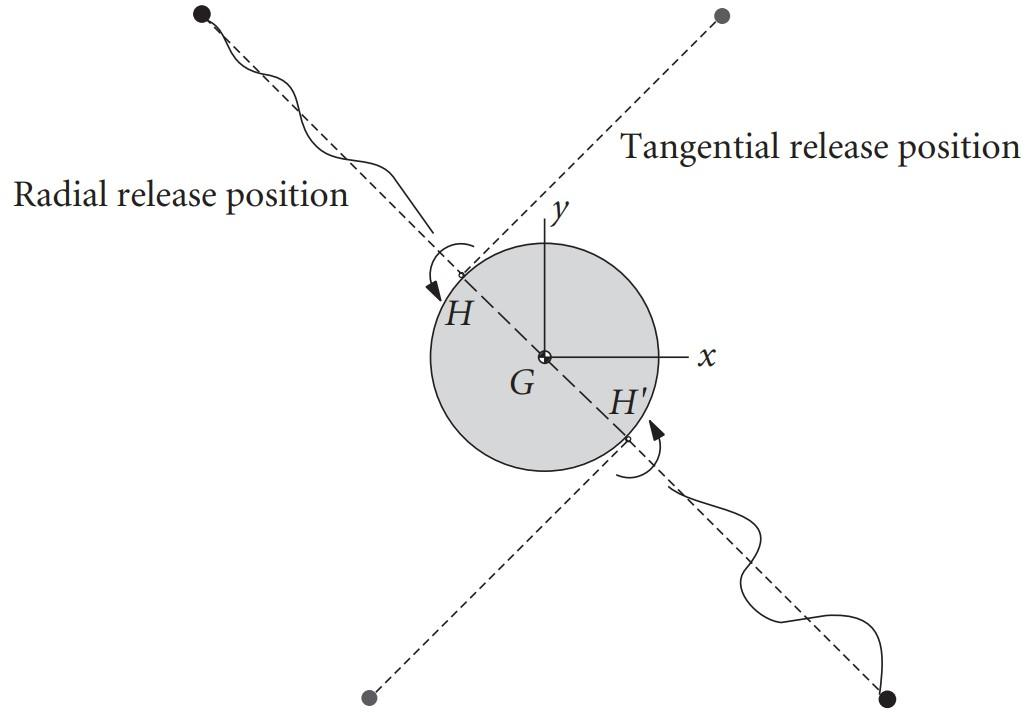
\includegraphics[width=0.75\linewidth]{images/tangential-radial}
    \caption{Comparison of radial and tangential release for a yo-yo despin system (from~\cite{curtis-orbital-mech})}
    \label{figure:tangential-radial}
\end{figure}


\begin{figure}
    \centering
    \begin{tikzpicture}
        \begin{axis}[
            width=12cm,
            height=9cm,
            xlabel={Combined Yo-Yo Despin Mass (kg)},
            ylabel={Cable Length (m)},
            xmin=0.0, xmax=0.4,
            ymin=0.0, ymax=1.6,
            xtick={0.0, 0.05, 0.1, 0.15, 0.2, 0.25, 0.3, 0.35, 0.4},
            xticklabels={0.0, 0.05, 0.1, 0.15, 0.2, 0.25, 0.3, 0.35, 0.4},
            ytick={0.0, 0.2, 0.4, 0.6, 0.8, 1.0, 1.2, 1.4, 1.6},
            yticklabels={0.0, 0.2, 0.4, 0.6, 0.8, 1.0, 1.2, 1.4, 1.6},
            xmajorgrids=true,
            ymajorgrids=true,
            y tick label style={
                font=\small,
                /pgf/number format/.cd,
                    fixed,
                    fixed zerofill,
                    precision=1,
                /tikz/.cd
            },
            x tick label style={
                font=\small,
                /pgf/number format/.cd,
                    fixed,
                    fixed zerofill,
                    precision=2,
                /tikz/.cd
            }
        ]
            \addplot+[
                no marks,
                line width=2pt,
            ]
            table{data/tangent.csv};
            \addplot+[
                no marks,
                line width=2pt,
            ]
            table{data/radial.csv};
            \legend{Tangential Release, Radial Release}
        \end{axis}
    \end{tikzpicture}
    \caption{Tradeoff between yo-yo despin masses and cable length}
    \label{figure:yoyo-plots}
\end{figure}

\Cref{figure:yoyo-plots} shows the required cable length, as a function of the yo-yo mass, to de-spin the vehicle completely. This analysis makes conservative assumptions: a stage dry mass of 10 kg, distributed as a cylindrical shell, and a 4 inch diameter. The relationship proves the feasibility of this mechanism for our mission.
